%! Author = Denis Moraes Guimarães
%! Date = 21/05/2026

\begin{frame}{Níveis de teste - Teste de integração de componentes}
    \begin{itemize}
        \item Teste das interfaces e interações entre os componentes.
        \item Depende muito das abordagens da estratégia de integração, como bottom-up, top-down ou big-bang. 
        \item Normalmente, são realizados por desenvolvedores em seus ambientes de desenvolvimento.
        \item É desenvolvido driver ou stub para simular o comportamento de componentes que ainda não foram integrados.
    \end{itemize}
    \vspace{0.5cm}
    \centering
    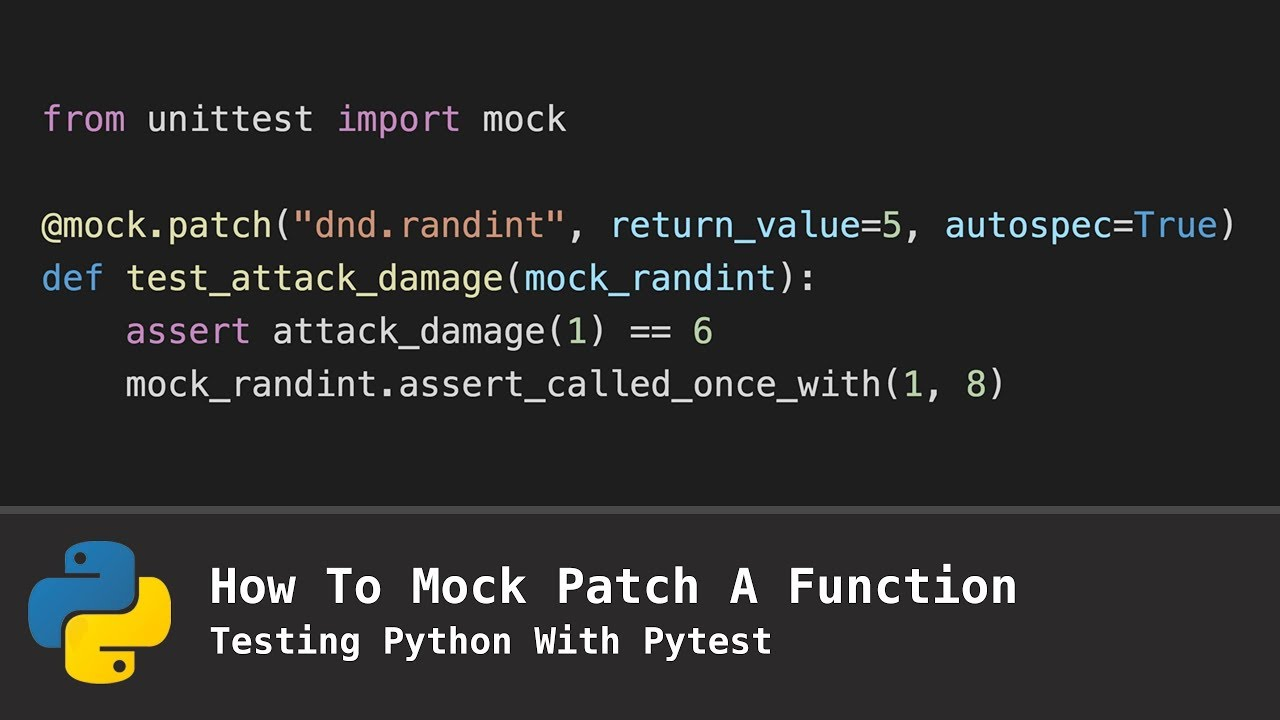
\includegraphics[width=0.8\textwidth]{images/mock.jpg}
\end{frame}